

\section{How is the channel number coverted into angle?}\label{sec:angcal}


%\begin{figure}[!h]
%\centering 
%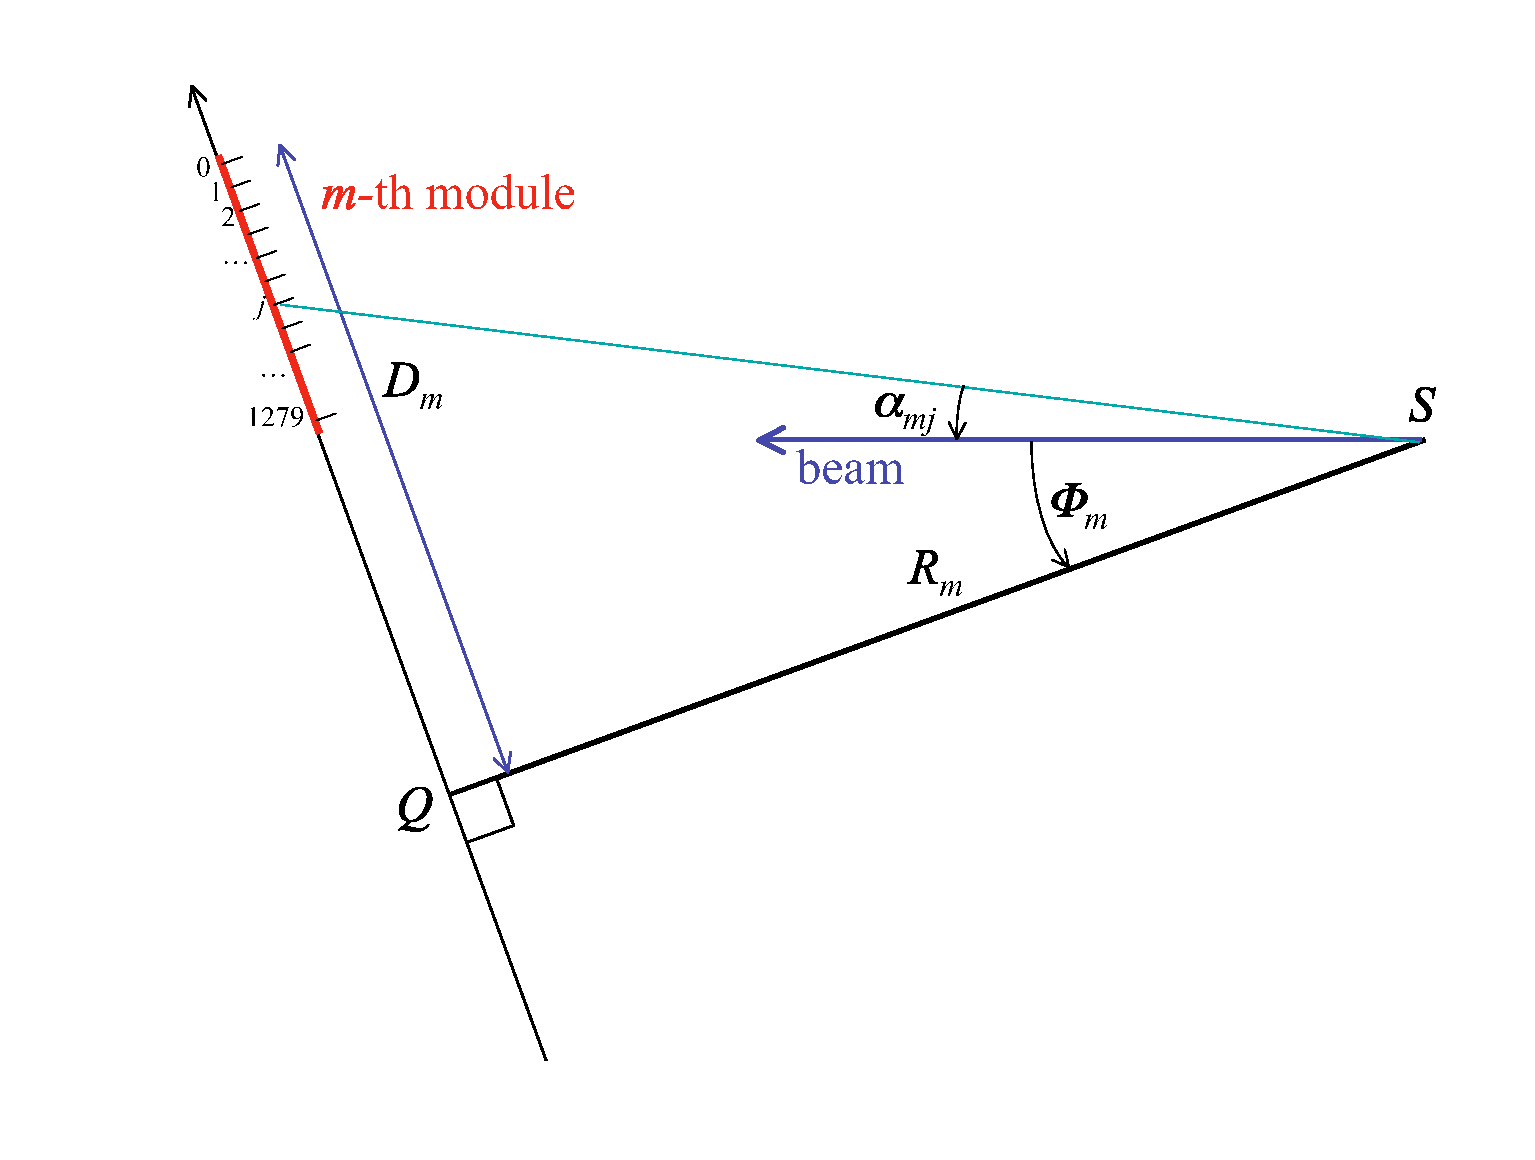
\includegraphics[width=0.98\textwidth]{AngConv}
%\caption{Schematics of the scattering geometry in the diffraction plane. A Mythen II module is shown. $R_m$ is the distance from the module sensor plane (orthogonal to the diffraction plane) to the sample position $S$; $D_m$ the distance from the center of pixel $j=0$ to point $Q$, counted positively as the arrow on the module plane goes (\emph{i.e.}, oppositely to the direction of increasing $j$); $\Phi_m$ is the angle of the module plane normal with the beam direction, positive counterclockwise. $\alpha_{jm}$ is the angular position of the $j$-th pixel center with respect to the beam direction, positive counterclockwise.}
%\label{acon}
%\end{figure}

Mythen II modules are composed by 1280 pixels, each having width p=0.05~mm, and numbered with j=0,..,1279. 
Angles are counted counterclockwise from the beam direction. For the m-th module, the angle $\alpha_{jm}$ of its j-th pixel center 
can be determined using the three geometric parameters $R_m$~[mm], $\Phi_m$~[deg], $D_m$~[mm], as in \fref{acon}. 
The detector group uses instead the 3 parameters center $c_m$~[\ ], offset $o_m$~[deg], conversion $k_m$~[\ ]. 
The law with the 3 geometric parameter is
\begin{equation}
\alpha_{jm}=\Phi_m-\lrb{\DSF{180}{\pi}}\arctan\lrb{\DSF{D_m-pj}{R_m}}
\end{equation}
The corresponding law using DG's parameters is
\begin{equation}
\alpha_{jm}=o_m+\lrb{\DSF{180}{\pi}}c_mk_m+\lrb{\DSF{180}{\pi}}\arctan\lrs{\lrb{j-c_m}k_m}
\end{equation}
One can convert the two forms by equating separately the term out of the arctan and the argument of arctan for two different values of j. 
It results
\begin{eqnarray}
c_m&=&\DSF{D_m}{p};\\ 
k_m&=&\DSF{p}{R_m};\\ 
o_m&=&\Phi_m-\DSF{180}{\pi}\DSF{D_m}{R_m}.
\end{eqnarray}
Conversely,
\begin{eqnarray}
\Phi_m&=&o_m+\DSF{180}{\pi}c_mk_m;\\
R_m&=&\DSF{p}{k_m};\\
D_m&=&c_m p.
\end{eqnarray}

\section{How are different positions merged together?}\label{sec:merging}



\subsection{Introduction}
\subsubsection{Notation}

[I use symbol $\TT$ for the diffraction angle $2\theta$]

\subsubsection{Observables}
The physical observable of interest in any scattering experiment is [1-3] the differential cross section
\[
\DSF{\DD{}\bf{\sigma}}{\DD{}\Omega}
\]
as a function of direction $\Omega$. 
To measure that directly we should operate with zero-width point detectors, with instant measurement and unit incident intensity. 
Practically 
the quantity we can actually measure - putting a detector in a position covering a certain 
solid angle for a certain time with a certain incident intensity - is
\[
{I_0}\Delta t \Delta\Omega\DSF{\DD{}\bf{\sigma}}{\DD{}\Omega}
\]
If $\Delta t$, $\Delta\Omega$ are small and known and $I_0$ is separately monitored, 
we can (have to) normalize the observations by simply dividing them out. 

Specifically for the powder diffraction field, historically, this is not usually done because
- as it is normally true with anode sources and point detectors and usual procedures - 
the counting times $\Delta t$, the solid angle width $\Delta\Omega\propto \Delta \TT$ 
and the incident intensity $I_0$ are considered 
constant and therefore go into some 'global scaling' constant that is usually considered arbitrary. 

However, as we have more sophisticated acquisition methods, 
we may need revert to the original approach and consider the 
counts divided by time and angular width as the real observable.

\subsection{Basic binning}\label{sec:11}

\begin{itemize}
\item[1.\ ]{
We have several patterns, say $P$. Each $k$-th pattern, for $k=1,\ldots,P$, is
constituted by $N_k$ angular intervals in the diffraction angle $2\theta\equiv\TT$:
\[
b_{k,j}=\lrs{\TT_{k,j}^{-},\TT_{k,j}^{+}},\qquad j=1,\ldots,N_k
\]
of center
\[
\hat{b}_{k,j}=\DSF{\TT_{k,j}^{+}+\TT_{k,j}^{-}}{2}
\]
and width
\[
\lrv{b_{k,j}}=\TT_{k,j}^{+}-\TT_{k,j}^{-}
\]
To each interval is associated a counting $C_{k,j}$, an efficiency correction factor $e_{k,j}$, a 
monitor $m_{k,j}$ (ionization chamber times acquisition time). All 'bad' intervals have been already flagged down and discarded.
Efficiency corrections and monitors are supposed to be normalized to a suitable value. 
Note that intervals $b_{k,j}$ might have multiple overlaps and might not cover an compact angular
range. }
%
\item[2.\ ]{Following Mighell's statistics[6] and normal scaling procedures, we first 
transform those numbers into associated intensities, intensity rates and relevant s.d.:
\[
I_{k,j}=\DSF{e_{k,j}}{m_{k,j}}\lrb{C_{k,j}+\min\lrb{1,C_{k,j}}}
\]
\[
\sigma_{I_{k,j}}=\DSF{e_{k,j}}{m_{k,j}}\sqrt{\lrb{C_{k,j}+1}}
\]
\[
r_{k,j}=\DSF{I_{k,j}}{\lrv{b_{k,j}}}=\DSF{e_{k,j}}{m_{k,j}\lrv{b_{k,j}}}\lrb{C_{k,j}+\min\lrb{1,C_{k,j}}}
\]
\[
\sigma_{r_{k,j}}=\DSF{\sigma_{I_{k,j}}}{\lrv{b_{k,j}}}=\DSF{e_{k,j}}{\lrv{b_{k,j}}m_{k,j}}\sqrt{\lrb{C_{k,j}+1}}
\]
 }
\item[3.\ ]{
We set up the final binned grid, 
composed of $M$ binning intervals
\[
B_\ell=[\TT_0+(\ell-1)B, \TT_0+\ell B],\qquad \ell=1,\ldots,M
\]
all contiguous and each having the same width \[\lrv{B_\ell}=B\] and each centered in 
\[\hat{B}_\ell=\TT_0+(\ell-1/2)B,\] 
covering completely the angular range between $\TT_0$ and $\TT_{max}=\TT_0+MB$.
}
\item[4.\ ]{
For bin $\ell$, we consider only and all the experimental intervals 
\[
b_{k,j}\qquad\text{such\ that}\qquad \lrv{ b_{k,j}\cap B_\ell } > 0.
\]
More restrictively, one may require to consider only and all the experimental intervals 
\[
b_{k,j}\qquad\text{such\ that}\qquad \hat{b}_{k,j}\in B_\ell .
\]
}
\item[5.\ ]{
In order to estimate the rate in each $\ell$-th bin, 
we use all above selected rate estimates concerning bin $B_\ell$ and we get
a better one with the weighted average method. \\
In the  weighted average method, we suppose to have a number $N_E$ of estimates $O_n$ 
of the same observable $O$, 
each one with a known s.d. $\sigma_{O_n}$ and each (optionally) repeated with a frequency 
$\nu_n$. 
Then
\[
\langle O\rangle =\DSF{
\mathop{\sum}_{n=1}^{N_E}\nu_n
O_n\sigma_{O_n}^{-2}
}{
\mathop{\sum}_{n=1}^{N_E}\nu_n
\sigma_{O_n}^{-2}
}
\]
%
Clearly the place of the frequencies in our case can be taken by coefficients 
\[
\DSF{\lrv{ b_{k,j}\cap B_\ell }}{B}
\]
that weigh the $k,j$-th estimate by its relative extension within bin $B_\ell$.
}
\item[6.\ ]{
Now 
we can simply accumulate registers 
\[
X_\ell=\mathop{\sum_{k,j}}_{ \lrv{ b_{k,j}\cap B_\ell } > 0}
\DSF{\lrv{ b_{k,j}\cap B_\ell }}{B}\  r_{k,j}\ \lrb{\sigma_{r_{k,j}}}^{-2}
\]
and 
\[
Y_\ell=\mathop{\sum_{k,j}}_{ \lrv{ b_{k,j}\cap B_\ell } > 0}
\DSF{\lrv{ b_{k,j}\cap B_\ell }}{B}\  \lrb{\sigma_{r_{k,j}}}^{-2}
\]
so that we can extract an intensity rate estimate (counts per unit diffraction angle and per unit time at constant incident intensity) as
\[
R_\ell=\DSF{X_\ell}{Y_\ell};
\]
\[
\sigma_{R_\ell}=\DSF{1}{\sqrt{Y_\ell}}.
\]
Now optionally we can transforms rates in intensities (multiplying 
both $R_\ell$ and $\sigma_{R_\ell}$ by $B$).
We can use any other scaling factor $K$ as we wish instead of $B$.  
The best cosmetic scaling is the one where
\[
\mathop{\sum}_{\ell=1}^M\DSF{KR_\ell}{K^2\sigma_{R_\ell}^2}=
\DSF{1}{K}
\mathop{\sum}_{\ell=1}^M\DSF{R_\ell}{\sigma_{R_\ell}^2}=M
\]
as if the intensities were simply counts. 
Therefore $K$ is given by
\[
K=\DSF{
1
}{
M
}\mathop{\sum}_{\ell=1}^M\DSF{R_\ell}{\sigma_{R_\ell}^2}
\]

In output then we give 3-column files 
with columns
\[
\hat{B}_\ell, \quad KR_\ell, \quad K\sigma_{R_\ell}
\]
}
\end{itemize}

\subsubsection{Special nasty cases}

Here we explore some special cases to see the robustness 
of the method. 

1) If no experimental observation contributes to bin $B_\ell$ according to one of the criteria
above, then we shall find $X_\ell=0$ and especially $Y_\ell=0$. The latter condition is 
valid as an exclusion condition 
(meaning that we discard that point and we do not perform further operations on it, 
neither do we output it).

2) if only one experimental observation - call it interval $b$, dropping indices - contributes 
to bin $B_\ell$, 
then we have 
\[
X_\ell=\DSF{\lrv{ b\cap B_\ell }}{B}\  
\DSF{e(C+1)}{m|b|}\ 
\lrb{
\DSF{|b|m}{e\sqrt{C+1}}
}^{2}
=\DSF{\lrv{ b\cap B_\ell }}{B}\DSF{|b|m}{e}
\]
\[
Y_\ell=\DSF{\lrv{ b\cap B_\ell }}{B}\  
\lrb{
\DSF{|b|m}{e\sqrt{C+1}}
}^{2}
=\DSF{\lrv{ b\cap B_\ell }}{B}\DSF{|b|^2m^2}{e^2(C+1)}
\]
and so
\[
R_\ell=\DSF{X_\ell}{Y_\ell}=\DSF{e(C+1)}{m|b|}
\]
that is the experimental rate as in pixel $b$;
\[
\sigma_{R_\ell}=\DSF{1}{\sqrt{Y_\ell}}=
\sqrt{\DSF{B}{\lrv{ b\cap B_\ell }}}
%
\DSF{e\sqrt{(C+1)}}{|b|m}
\]
that is the same s.d. that can be calculated directly for $b$, augmented by factor 
\[
\sqrt{\DSF{B}{\lrv{ b\cap B_\ell }}}
\]
that takes into account the extrapolation error.

\subsection{Advanced binning}\label{sec:2}

There are more advanced (and more complex) methods that take more carefully into account the real position of the centers $\hat{b}_{j,k}$ w.r.t. $\hat{B}_\ell$. 
If we find out that it is the case we may develop them too. 


\subsection{Poisson and normal statistics for diffraction}

The normal situation for diffraction data 
is that the observed signal is a photon count. 
Therefore it follows a Poisson distribution. 
If we have a count value $C_0$ that follows a Poisson distribution, 
we can assume immediately that the average is equal to $C_0$ and the s.d. is $\sqrt{C_0}$. 
I.e., repeated experiments would give values $n$ 
distributed according to the normalized distribution
\[
P(n)=\DSF{C_0^n\EE^{-C_0}
}{
n!}
\]
This obeys
\[
\mathop{\sum}_{n=0}^{+\infty}
P(n)=1\ ;
\]
\[
\langle n\rangle=\mathop{\sum}_{n=0}^{+\infty}
nP(n)=C_0\ ;
\]
\[
\langle n^2\rangle=\mathop{\sum}_{n=0}^{+\infty}
n^2 P(n)=C_0^2+C_0\ ;
\]
The standard deviation comes then to
\[
\sigma_{C_0}=\sqrt{\langle n^2\rangle-\langle n\rangle^2}=\sqrt{C_0}
\]

When the data have to be analyzed, one must compare observations with a model 
which gives calculated values of the observations in dependence of a certain set of 
parameters. The best values of the parameters (the target of investigation) 
are the one that maximize the likelihood function [4,5]. The likelihood function for 
Poisson variates is pretty difficult to use; furthermore, even simple data manipulations 
are not straightforward with Poisson variates (see \sref{sec:3}). The common choice is to approximate 
Poisson variates with normal variates, and then use the much easier formalism 
of normal distribution to a) do basic data manipulations and b) fit data with model. 
To the latter task, in fact, the likelihood function is maximized simply by minimizing 
the usual weighted-$\chi^2$[4] :
\[
\chi^2 = \mathop{\sum}_{j=1}^{N_{\mathrm{obs}}}
\DSF{\lrb{F_j-O_j}^2
}{
\sigma_j^2
}
\]
where $O_j$ are the experimentally observed values, $F_j$ the calculated model values, 
$\sigma_j$ the s.d.s of the observations.

Substituting directly the counts (and derived s.d.s) for the observations in the former :
\[
\chi_{(0)}^2 = \mathop{\sum}_{j=1}^{N_{\mathrm{obs}}}
\DSF{\lrb{F_j-C_j}^2
}{
C_j
}
\]
is the most common way. It is \emph{slightly} wrong to do so, however [6], 
the error being large only when the counts are low. 
There is also a divergence for zero counts. 
In fact, a slightly modified form [6] exists, reading
\[
\chi_{(1)}^2 = \mathop{\sum}_{j=1}^{N_{\mathrm{obs}}}
\DSF{\lrb{F_j-\lrb{C_j+\min\lrb{1,C_j}}}^2
}{
C_j+1
}
\]
Minimizing this form of $\chi^2$ is equivalent - to an exceptionally good approximation [6]- 
to maximizing the proper Poisson-likelihood. 











\subsection{Average vs. weighted average}

\subsubsection{Simple average}

Suppose we have $N_{\mathrm{obs}}$ Poisson-variate experimental evaluations 
$C_j,\quad j=1\ldots N_{\mathrm{obs}}$, 
of the same quantity $x$.
There are different ways to obtain from all $N_{\mathrm{obs}}$ data values a single estimate of the observable which is better than 
any of them. The most straightforward and the best is the simple average
\[
x=\langle x\rangle=\DSF{1}{ N_{\mathrm{obs}}}
 \mathop{\sum}_{j=1}^{N_{\mathrm{obs}}}C_j\ .
\]
As the sum of Poisson variates is a Poisson variate, the standard deviation 
\[
\sigma_x=\sqrt{\langle x^2\rangle-\langle x\rangle^2}=\sqrt{
\DSF{1}{ N_{\mathrm{obs}}}
 \mathop{\sum}_{j=1}^{N_{\mathrm{obs}}}C_j^2-\lrb{
 \DSF{1}{ N_{\mathrm{obs}}}
 \mathop{\sum}_{j=1}^{N_{\mathrm{obs}}}C_j
 }
 }
\]
can be evaluated more comfortably as
\[
\sigma_x=\DSF{1}{ N_{\mathrm{obs}}}\sqrt{  \mathop{\sum}_{j=1}^{N_{\mathrm{obs}}}C_j }
=\sqrt{\DSF{\langle x\rangle}{N_{\mathrm{obs}}}}
\]


\subsubsection{Zero-skipping average}

In some cases, in order to avoid possible singularities, 
values $C_j=0$ are skipped. Then if $N_{\mathrm{obs}}^*$ is the number of non-zero data points,
we can evaluate the 'zero-skipping' average as
\[
x=\langle x\rangle^*=\DSF{1}{ N_{\mathrm{obs}}^*}
 \mathop{\sum}_ {\stackrel{1\leqslant j\leqslant N_{\mathrm{obs}}}{{C_j>0}}}
 C_j=\DSF{1}{ N_{\mathrm{obs}}^*}
 \mathop{\sum}_{j=1}^{N_{\mathrm{obs}}}C_j = \DSF{N_{\mathrm{obs}}}{N_{\mathrm{obs}}^*}\langle x\rangle
\]
The standard deviation is then
\[
\sigma_{x^*}= \DSF{N_{\mathrm{obs}}}{N_{\mathrm{obs}}^*}\sigma_x = \sqrt{\DSF{N_{\mathrm{obs}}}{N_{\mathrm{obs}}^*}}
\sqrt{\DSF{\langle x\rangle}{N_{\mathrm{obs}}^*}}=\sqrt{\DSF{\langle x\rangle^*}{N_{\mathrm{obs}}^*}}
\]
Note that the s.d. is evaluated exactly as if the non-zero $C_j$ were the only observations, 
whilst the average is overestimated by the fraction of zero-counting events.

\subsubsection{Weighted average: definition and relationship with $\chi^2$}

A weighted average is the result of the special case of a data fitting to a model function which is a constant.
It is easy to see that minimizing w.r.t $x$
\[
\chi^2 = \mathop{\sum}_{j=1}^{N_{\mathrm{obs}}}
\DSF{\lrb{x-O_j}^2
}{
\sigma_j^2
}
\]
yields
\[
x= \langle x \rangle_{\!\mathrm{w}}=\DSF{
\mathop{\sum}_{j=1}^{N_{\mathrm{obs}}}
\DSF{O_j
}{
\sigma_j^2
}
}{
\mathop{\sum}_{j=1}^{N_{\mathrm{obs}}}
\DSF{1
}{
\sigma_j^2
}
}
\]
The good-faith s.d. (square-root of twice the inverse of the second derivative of $\chi^2$ at the minimum) 
is then
\[
\sigma_{\langle x \rangle_{\!\mathrm{w}}} = \DSF{
1
}{\sqrt{
\mathop{\sum}_{j=1}^{N_{\mathrm{obs}}}
\DSF{1
}{
\sigma_j^2
}
}}
\]
I use the term 'good-faith' to indicate the case when it is really appropriate to use a constant as a model functions, 
i.e. when the observations are truly different observations of the same observable. 
When this is not the case but we do not know what to do better we can at least increase the s.d. 
In fact, there is a correction factor for the s.d., given - in this case - by
\[
\mathsf{GoF}=
\sqrt{
\DSF{
\mathop{\sum}_{j=1}^{N_{\mathrm{obs}}}
\DSF{O_j^2
}{
\sigma_j^2
}
-\DSF{
\lrs{
\mathop{\sum}_{j=1}^{N_{\mathrm{obs}}}
\DSF{O_j
}{
\sigma_j^2
}
}^2
}{ \mathop{\sum}_{j=1}^{N_{\mathrm{obs}}}
\DSF{1
}{
\sigma_j^2
} }
}{
N_{\mathrm{obs}}-1
}
}
\]
so that
\[
{\sigma}_{\langle x \rangle_{\!\mathrm{w}}}^{\mathrm{corrected}} = \mathsf{GoF}\ \sigma_{\langle x \rangle_{\!\mathrm{w}}}
\] 

Specializing now to the two cases above, 

\subsubsection{Straight Poisson (zero-skipping) weighted average}

When $O_j=C_j$ and $\sigma_j^2=C_j$
\[
\langle x \rangle_{\!\mathrm{w(1)}}=\DSF{
{N_{\mathrm{obs}}}
}{
\mathop{\sum}_{j=1}^{N_{\mathrm{obs}}}
\DSF{1
}{
C_j
}
}
\]
Here we need to eliminate the singularity when $C_j=0$. In order to do so, we skip data points which are zero. 
Then if $N_{\mathrm{obs}}^*$ is the number of non-zero data points, 
\[
\langle x \rangle_{\!\mathrm{w(1)}}=\DSF{
{N_{\mathrm{obs}}^*}
}{
\mathop{\sum}_{\stackrel{1\leqslant j\leqslant N_{\mathrm{obs}}}{{C_j>0}}}
\DSF{1
}{
C_j
}
}
\]
\[
\sigma_{\langle x \rangle_{\!\mathrm{w(1)}}} = \DSF{
1
}{\sqrt{
\mathop{\sum}_{\stackrel{1\leqslant j\leqslant N_{\mathrm{obs}}}{{C_j>0}}}
\DSF{1
}{
C_j
}
}}=\sqrt{\DSF{\langle x \rangle_{\!\mathrm{w(1)}}}{
N_{\mathrm{obs}}^*
}}
\]
\[
\mathsf{GoF}_{(1)}=
\sqrt{
\DSF{
\mathop{\sum}_{\stackrel{1\leqslant j\leqslant N_{\mathrm{obs}}}{{C_j>0}}}
\!\!\!\!C_j
%
-\DSF{
\lrs{
N_{\mathrm{obs}}^*
}^2
}{ \mathop{\sum}_{\stackrel{1\leqslant j\leqslant N_{\mathrm{obs}}}{{C_j>0}}}
\DSF{1
}{
C_j
} }
}{
N_{\mathrm{obs}}^*-1
}
}
=\sqrt{
\DSF{N_{\mathrm{obs}}^*}{N_{\mathrm{obs}}^*-1}
\lrb{
\langle x\rangle^*-\langle x \rangle_{\!\mathrm{w(1)}}
}
}
\]
where $\langle x\rangle^*$ is the simple average of the non-zero data points; and of course
\[
{\sigma}_{\langle x \rangle_{\!\mathrm{w(1)}}}^{\mathrm{corrected}} = \mathsf{GoF}_{(1)}\ \sigma_{\langle x \rangle_{\!\mathrm{w(1)}}}
\] 

\subsubsection{Mighell-Poisson weighted average}

When $O_j=C_j+\min\lrb{1,C_j}$ and $\sigma_j^2=C_j+1$
\[
\langle x \rangle_{\!\mathrm{w(2)}}=\DSF{
{N_{\mathrm{obs}}^*}
}{
\mathop{\sum}_{\stackrel{1\leqslant j\leqslant N_{\mathrm{obs}}}{{C_j>0}}}
\DSF{1
}{
C_j+1
}
}
\]
\[
\sigma_{\langle x \rangle_{\!\mathrm{w(2)}}} = \DSF{
1
}{\sqrt{
\mathop{\sum}_{\stackrel{1\leqslant j\leqslant N_{\mathrm{obs}}}{{C_j>0}}}
\DSF{1
}{
C_j+1
}
}}=\sqrt{\DSF{\langle x \rangle_{\!\mathrm{w(2)}}}{
N_{\mathrm{obs}}^*
}}
\]
\[
\mathsf{GoF}_{(2)}=
\sqrt{
\DSF{
\mathop{\sum}_{\stackrel{1\leqslant j\leqslant N_{\mathrm{obs}}}{{C_j>0}}}
\!\!\!\!C_j+N_{\mathrm{obs}}^*
%
-\DSF{
\lrs{
N_{\mathrm{obs}}^*
}^2
}{ \mathop{\sum}_{\stackrel{1\leqslant j\leqslant N_{\mathrm{obs}}}{{C_j>0}}}
\DSF{1
}{
C_j+1
} }
}{
N_{\mathrm{obs}}^*-1
}
}
=\sqrt{
\DSF{N_{\mathrm{obs}}^*}{N_{\mathrm{obs}}^*-1}
\lrb{
\langle x\rangle^*-\langle x \rangle_{\!\mathrm{w(2)}}+1
}
}
\]
where $\langle x\rangle^*$ is the simple average of the non-zero data points; and of course
\[
{\sigma}_{\langle x \rangle_{\!\mathrm{w(2)}}}^{\mathrm{corrected}} = \mathsf{GoF}_{(2)}\ \sigma_{\langle x \rangle_{\!\mathrm{w(2)}}}
\] 






\subsubsection{Comparison}

We have seen four different ways to take an average -
two simple averages (the second skipping zero values) 
and two weighted averages (using straight Poisson and Poisson-Mighell [6] $\chi^2$ formulations). 
We know that the simple average (not skipping zeros) is the best possible result. However, 
there are inconveniences with it. If for instance we need to scale our data before averaging, then the 
simple average is no more usable (it will give the correct average but a bad estimate of the s.d.) .
In any case, the passage to normal statistics (using Mighell's correction) needs to be done before or later. 
Therefore a comparison is due in order to ascertain 
how wrong can it be using the different methods. 

We have to give a measure of what is negligible first. 
The relative error is a measure of the smallest relative variation of an estimate $x$ that is \emph{not} negligible:
\[
\epsilon_x = \DSF{\sigma_x}{x}
\]
We shall then consider negligible 
(w.r.t. $x$) terms whose relative magnitude is $O(\epsilon_x^2)$.
As the s.d. of $x$ is $\propto\epsilon_x$, we may not discard terms $O(\epsilon_x^2)$ on the s.d.; 
there instead we may neglect terms $O(\epsilon_x^3)$.


\subsubsection{Analytical comparison of averages}

First we give an analytical comparison between simple average and Mighell-Poisson weighted average 
for $N_{\mathrm{obs}}=2$. 
If the two events are $C_1$ and $C_2$, then
\[
\langle x \rangle=\DSF{C_1+C_2}{2}; \qquad \sigma_x=\DSF{\sqrt{C_1+C_2}}{2}
\]
For the M-P weighted average,
\[
\langle x \rangle_{\mathrm{w(2)}}=\DSF{2(C_1+1)(C_2+1)}{C_1+C_2+2}; \qquad 
\sigma_{\langle x \rangle_{\mathrm{w(2)}}}=\sqrt{\DSF{(C_1+1)(C_2+1)}{C_1+C_2+2}}
\]

Now, supposing that the common 'true' value of $C_1,C_2$ is $\lambda$, 
we use the Poisson distribution to compare the expectation values of the two results. The expectation value of the simple average is
\[
E\lrb{\langle x \rangle} = \mathop{\sum}_{m,n=0}^{+\infty}
 \DSF{n+m}{2}P(n)P(m)=\mathop{\sum}_{m=0}^{+\infty}
 \DSF{m}{2}\DSF{\lambda^m\EE^{-\lambda}}{m!}
 +\mathop{\sum}_{n=0}^{+\infty}
 \DSF{n}{2}\DSF{\lambda^n\EE^{-\lambda}}{n!}
 =\lambda
\]
As expected, the simple average gives the true value. 
For its variance, 
\[
E\lrb{\sigma_x^2} = \mathop{\sum}_{m,n=0}^{+\infty}
 \DSF{n+m}{4}P(n)P(m)=\DSF{
 \lambda}{2};\qquad E\lrb{\sigma_x} =\sqrt{\DSF{\lambda}{2}}
\]


In order to evaluate the difference with the M-P weighted average, we rewrite the latter as
\[
\langle x \rangle_{\mathrm{w(2)}}=\langle x \rangle + 1 -\DSF{(C_1-C_2)^2}{4(\langle x \rangle+1)}
\]
and calculate the expectation value of the last term:
\[
E\lrb{\DSF{(C_1-C_2)^2}{4(\langle x \rangle+1)}} = 
 \mathop{\sum}_{m,n=0}^{+\infty}
 \DSF{(n-m)^2}{2(n+m+2) }P(n)P(m)=\DSF{\EE^{-2\lambda}}{2}
 \mathop{\sum}_{m,n=0}^{+\infty}
 \DSF{(n-m)^2}{(n+m+2) }\DSF{\lambda^{n+m}}{n!m!}
\]
Rearranging the sums with $s=n+m$, $s=0\ldots +\infty$; $n-m=s-2k$, $k=0\ldots s$,
we get
\[
E\lrb{\DSF{(C_1-C_2)^2}{4(\langle x \rangle+1)}} = 
\DSF{\EE^{-2\lambda}}{2}
 \mathop{\sum}_{s=0}^{+\infty}
  \mathop{\sum}_{k=0}^{s}
 \DSF{(s-2k)^2(s+1)}{(s+2)! }{\lambda^{s}}
 \binom{s}{k}=\DSF{1}{2}-\DSF{1}{2\lambda}+\DSF{1-\EE^{-2\lambda}}{4\lambda^2}
 %{n!m!}
\]
So, the relative difference between averages is
\[
\DSF{E\lrb{\langle x \rangle_{\mathrm{w(2)}}-\langle x \rangle}}{E\lrb{\langle x \rangle}}=
\DSF{1}{2\lambda}+\DSF{1}{2\lambda^2}-\DSF{1-\EE^{-2\lambda}}{4\lambda^3}
\]
The relative error on $\langle x \rangle$ is
\[
\epsilon = \DSF{\sigma_x}{\langle x \rangle} = 
\DSF{\lambda^{1/2}}{\sqrt{2} \lambda}=\DSF{1}{\sqrt{2\lambda}}
\]
therefore 
\[
\DSF{E\lrb{\langle x \rangle_{\mathrm{w(2)}}-\langle x \rangle}}{E\lrb{\langle x \rangle}}=
O(\epsilon^2)
\]
Therefore, the expectation value of the error (relative) involved in taking 
the M-P weighted average instead of the simple average is negligible.



\subsubsection{Numerical comparison of averages}

In the next table numerical results are displayed. An exact random-Poisson generator has been used to generate Poisson deviates of given average value 
$\lambda$, with $\lambda=1,10,100,\ldots,1000000$. For each value $\lambda$
$N=10^8$ deviates have been generated. Then averages have been taken for each value $\lambda$ and compared with the true value. 
For each value $\lambda$ - in order to have a scale for comparison - 
we evaluate the expected absolute s.d. of averages as $\xi_\lambda=\sqrt{\lambda/N}$, and the relative s.d. of averages as $\epsilon_\lambda=\sqrt{\lambda/N}/\lambda=1/\sqrt{N\lambda}$. Then - for each averaging method - we evaluate the error $E_\lambda$ (average minus $\lambda$), 
the relative error $e_\lambda=E_\lambda/\lambda$, and finally the comparison criterion $e_\lambda/\epsilon_\lambda$ (bold). The comparison criterion is expected to be close to 1 in absolute value. Values much larger than one mean that we are introducing a systematic error.

\footnotesize

\begin{tabular}{l|llll}
\footnotesize
% # trials N =  100000000
\ &&&&\ \\
& \multicolumn{4}{l}{$\lambda =$  1. ; $\xi_\lambda = $0.0001 ; $\epsilon_\lambda$ =  0.0001}\\
 & ${\langle x \rangle_{\!\mathrm{w(1)}}}$  &  ${\langle x \rangle_{\!\mathrm{w(2)}}}$  &  $\langle  x \rangle^*$ &  $\langle  x \rangle$\\
Averages & 1.303772380383934  &  0.9999155361216990  &  1.581941754994651  &  0.9999283300000000    \\
$E_\lambda$ & 0.3037723803839338  &  -0.8446387830096658E-04  &  0.5819417549946508  &  -0.7166999999996815E-04\\
$e_\lambda$ & 0.3037723803839338  &  -0.8446387830096658E-04  &  0.5819417549946508  &  -0.7166999999996815E-04\\
$e_\lambda/\epsilon_\lambda$ &{\textbf{ 3037.723803839338  }}&{\textbf{  -0.8446387830096658  }}&{\textbf{  5819.417549946508  }}&{\textbf{  -0.7166999999996815   }} \\
\ &&&&\ \\
 & \multicolumn{4}{l}{$\lambda =$  10.000000000000002 ; $\xi_\lambda = $0.00031622776601683794 ; $\epsilon_\lambda$ =  0.00003162277660168379}\\
  &  ${\langle x \rangle_{\!\mathrm{w(1)}}}$  &  ${\langle x \rangle_{\!\mathrm{w(2)}}}$  &  $\langle  x \rangle^*$  &  $\langle  x \rangle$\\
Averages & 8.848248847530357  &  10.00025732384808  &  10.00052232372917  &  10.00006800000000    \\
$E_\lambda$ & -1.151751152469645  &  0.2573238480785278E-03  &  0.5223237291644978E-03  &  0.6799999999884676E-04\\
$e_\lambda$ & -0.1151751152469645  &  0.2573238480785278E-04  &  0.5223237291644977E-04  &  0.6799999999884675E-05\\
$e_\lambda/\epsilon_\lambda$ &{\textbf{ -3642.156939527943  }}&{\textbf{  0.8137294562072904  }}&{\textbf{  1.651732660112730  }}&{\textbf{  0.2150348808878029 }}   \\
\ &&&&\ \\
 & \multicolumn{4}{l}{$\lambda =$  100.00000000000004 ; $\xi_\lambda = $0.0010000000000000002 ; $\epsilon_\lambda$ =  0.000009999999999999997}\\
  &  ${\langle x \rangle_{\!\mathrm{w(1)}}}$  &  ${\langle x \rangle_{\!\mathrm{w(2)}}}$  &  $\langle  x \rangle^*$  &  $\langle  x \rangle$\\
Averages & 98.98978896904168  &  100.0001037814804  &  100.0002153600000  &  100.0002153600000    \\
$E_\lambda$ & -1.010211030958359  &  0.1037814803765968E-03  &  0.2153599999559219E-03  &  0.2153599999559219E-03\\
$e_\lambda$ & -0.1010211030958359E-01  &  0.1037814803765968E-05  &  0.2153599999559218E-05  &  0.2153599999559218E-05\\
$e_\lambda/\epsilon_\lambda$ &{\textbf{ -1010.211030958359  }}&{\textbf{  0.1037814803765968  }}&{\textbf{  0.2153599999559219  }}&{\textbf{  0.2153599999559219  }}  \\
\ &&&&\ \\
 & \multicolumn{4}{l}{$\lambda =$  1000.0000000000007 ; $\xi_\lambda = $0.0031622776601683803 ; $\epsilon_\lambda$ =  0.000003162277660168378}\\
  &  ${\langle x \rangle_{\!\mathrm{w(1)}}}$  &  ${\langle x \rangle_{\!\mathrm{w(2)}}}$  &  $\langle  x \rangle^*$  &  $\langle  x \rangle$\\
Averages & 999.0029754507847  &  1000.003978305674  &  1000.003836760000  &  1000.003836760000    \\
$E_\lambda$ & -0.9970245492160075  &  0.3978305673513205E-02  &  0.3836759999330752E-02  &  0.3836759999330752E-02\\
$e_\lambda$ & -0.9970245492160069E-03  &  0.3978305673513202E-05  &  0.3836759999330750E-05  &  0.3836759999330750E-05\\
$e_\lambda/\epsilon_\lambda$ &{\textbf{ -315.2868458625229  }}&{\textbf{  1.258050715667192  }}&{\textbf{  1.213290043331128  }}&{\textbf{  1.213290043331128  }}  \\
\ &&&&\ \\
 & \multicolumn{4}{l}{$\lambda =$  10000.00000000001 ; $\xi_\lambda = $0.010000000000000005 ; $\epsilon_\lambda$ =  9.999999999999995E-7}\\
  &  ${\langle x \rangle_{\!\mathrm{w(1)}}}$  &  ${\langle x \rangle_{\!\mathrm{w(2)}}}$  &  $\langle  x \rangle^*$  &  $\langle  x \rangle$\\
Averages & 9998.995728116572  &  9999.995828163173  &  9999.995919900000  &  9999.995919900000    \\
$E_\lambda$ & -1.004271883437468  &  -0.4171836835666909E-02  &-0.4080100008650334E-02  &-0.4080100008650334E-02\\
$e_\lambda$ & -0.1004271883437467E-03 & -0.4171836835666905E-06 & -0.4080100008650330E-06  &-0.4080100008650330E-06\\
$e_\lambda/\epsilon_\lambda$ &{\textbf{ -100.4271883437468  }}&{\textbf{  -0.4171836835666907  }}&{\textbf{  -0.4080100008650331  }}&{\textbf{  -0.4080100008650331  }}  \\
\ &&&&\ \\
 & \multicolumn{4}{l}{$\lambda =$  100000.0000000002 ; $\xi_\lambda = $0.031622776601683826 ; $\epsilon_\lambda$ =  3.162277660168376E-7}\\
  &  ${\langle x \rangle_{\!\mathrm{w(1)}}}$  &  ${\langle x \rangle_{\!\mathrm{w(2)}}}$  &  $\langle  x \rangle^*$  &  $\langle  x \rangle$\\
Averages & 99999.01275394148  &  100000.0127639189  &  100000.0125627100  &  100000.0125627100    \\
$E_\lambda$ & -0.9872460587212117  &  0.1276391866849735E-01  &  0.1256270980229601E-01  &  0.1256270980229601E-01\\
$e_\lambda$ & -0.9872460587212097E-05  &  0.1276391866849733E-06  &  0.1256270980229599E-06  &  0.1256270980229599E-06\\
$e_\lambda/\epsilon_\lambda$ &{\textbf{ -31.21946156583365  }}&{\textbf{  0.4036305486159527  }}&{\textbf{  0.3972677655897895  }}&{\textbf{  0.3972677655897895   }} \\
\ &&&&\ \\
 & \multicolumn{4}{l}{$\lambda =$  1000000.0000000013 ; $\xi_\lambda = $0.10000000000000006 ; $\epsilon_\lambda$ =  9.999999999999993E-8}\\
  &  ${\langle x \rangle_{\!\mathrm{w(1)}}}$  &  ${\langle x \rangle_{\!\mathrm{w(2)}}}$  &  $\langle  x \rangle^*$  &  $\langle  x \rangle$\\
Averages & 999999.1188353101  &  1000000.118835812  &  1000000.118809340  &  1000000.118809340    \\
$E_\lambda$ & -0.8811646911781281  &  0.1188358106883243  &  0.1188093387754634  &  0.1188093387754634  \\
$e_\lambda$ & -0.8811646911781270E-06  &  0.1188358106883241E-06  &  0.1188093387754633E-06  &  0.1188093387754633E-06\\
$e_\lambda/\epsilon_\lambda$ &{\textbf{ -8.811646911781276  }}&{\textbf{  1.188358106883242  }}&{\textbf{  1.188093387754633  }}&{\textbf{ 1.188093387754633}} \\
 \end{tabular}

\normalsize

As it is visible from the table:
\begin{itemize}
\item[1.\quad]{${\langle x \rangle_{\!\mathrm{w(1)}}}\ :$ the weighted average using straight Poisson statistics is consistenty bad at all values of $\lambda$, that means at all counting levels;}
\item[2.\quad]{${\langle x \rangle^*}\ $:  the normal average skipping zero count data is bad for $\lambda<100$, that means at low counting levels (of course at higher counting levels zeroes are not happening);}
\item[3.\quad]{${\langle x \rangle}\ \text{and}\ {\langle x \rangle_{\!\mathrm{w(2)}}}$: the normal average including zero count data and the Mighell-Poisson weighted average 
are consistently and equivalently good at all counting levels.}
\end{itemize}
Therefore there is no bias when using the Mighell-Poisson weighted method to average data w.r.t. the usual average. The former, however, 
has already accomplished the passage to normal statistics, therefore all operations on data that are not simple averaging can be done in 
the framework of normal statistics, where everything is known and clear. In the next section, on the opposite, it is shown that 
even simple operations as scaling data lead to the necessity of abandoning Poisson statistics in order to estimate correctly the standard deviations.





\subsection{Scaling Poisson variates}\label{sec:3}

If we have a count value $C_0$ that follows a Poisson distribution, 
we can assume immediately that the average is $C_0$ and the s.d. is $\sqrt{C_0}$. 
I.e., repeated experiments would give values $n$ 
distributed according to the normalized distribution
\[
P(n)=\DSF{C_0^n\EE^{-C_0}
}{
n!}
\]
This obeys
\[
\mathop{\sum}_{n=0}^{+\infty}
P(n)=1\ ;
\]
\[
\langle n\rangle=\mathop{\sum}_{n=0}^{+\infty}
nP(n)=C_0\ ;
\]
\[
\langle n^2\rangle=\mathop{\sum}_{n=0}^{+\infty}
n^2 P(n)=C_0^2+C_0\ ;
\]
\[
\sigma_{C_0}=\sqrt{\langle n^2\rangle-\langle n\rangle^2}=\sqrt{C_0}
\]
Suppose now that
our observable is 
\[
X_0=\eta_0 C_0
\]
where $\eta_0$ is a known error-free scaling factor. 
The distribution of $X$ is
\[
P'(X)=P(X/\eta_0)=P(n)\qquad\Biggl|\Biggr.\qquad \frac{X}{\eta_0}\equiv n\in\mathbb{Z}
%=\left.\DSF{(X_0/\eta_0)^{X/\eta_0}\EE^{-X_0/\eta_0}}{(X/\eta_0)!}\right|_{\frac{X}{\eta_0}\in\mathbb{Z}}
\]
and now,
\[
\mathop{\sum}_{n=0}^{+\infty}
P(n)=1\ ;
\]
\[
\langle X\rangle=\mathop{\sum}_{n=0}^{+\infty}
\eta_0 nP(n)=\eta_0 C_0=X_0\ ;
\]
\[
\langle X^2\rangle=\mathop{\sum}_{n=0}^{+\infty}
\eta_0^2 n^2 P(n)=\eta_0^2(C_0^2+C_0)=X_0^2+\eta_0 X_0\ ;
\]
\[
\sigma_X=\sqrt{\langle X^2\rangle-\langle X\rangle^2}=\sqrt{\eta_0 X_0}=\eta_0\sqrt{C_0}=\sqrt{\eta_0}\sqrt{X_0}
\]
Now it is no more valid that $\sigma_X=\sqrt{\langle X\rangle}=\sqrt{X_0}$, instead
\[
\sigma_X=\sqrt{\eta_0}\sqrt{X_0}=\eta_0\sqrt{C_0}=\eta_0\sigma_{C_0}
\]
that is the characteristic relationship for a normal-variate distribution.

Moreover, assume now that the scaling factor is not exctly known 
but instead it is a normal-variate itself with average $\eta_0$, s.d. 
$\sigma_{\eta_0}$, and distribution
\[
\widehat{P}(\eta)=\DSF{
\EE^{
-\frac{1}{2}
\lrb{
\frac{\eta-\eta_0}{\sigma_{\eta_0}}
}^2
}
}{
\sigma_{\eta_0}\sqrt{2\pi}
}
\]
Then,
\[
\int_{-\infty}^{+\infty}\DD{\eta}\mathop{\sum}_{n=0}^{+\infty}
P(n)\widehat{P}(\eta)=1\ ;
\]
\[
\langle X\rangle=\int_{-\infty}^{+\infty}\DD{\eta}\mathop{\sum}_{n=0}^{+\infty}
\widehat{P}(\eta)\eta nP(n)=
\mathop{\sum}_{n=0}^{+\infty}
 nP(n)
\int_{-\infty}^{+\infty}\DD{\eta} \widehat{P}(\eta)\eta
 =
\eta_0 C_0=X_0\ ;
\]
\[
\langle X^2\rangle=\int_{-\infty}^{+\infty}\DD{\eta}\mathop{\sum}_{n=0}^{+\infty}
\widehat{P}(\eta)\eta^2 n^2 P(n)=
\int_{-\infty}^{+\infty}\DD{\eta}\widehat{P}(\eta)\eta^2
\mathop{\sum}_{n=0}^{+\infty}
 n^2 P(n)
=
(\eta_0^2+\sigma_{\eta_0}^2)(C_0^2+C_0)\ ;
\]
\[
\DSF{\sigma_X}{\langle X\rangle}=\DSF{\sqrt{\langle X^2\rangle-\langle X\rangle^2}}{\langle X\rangle}
=\DSF{\sqrt{
\eta_0^2 C_0+\sigma_{\eta_0}^2C_0^2+\sigma_{\eta_0}^2 C_0
}}{\eta_0C_0}=
\sqrt{
\lrb{\DSF{ \sigma_{C_0}}{C_0}}^2
+\lrb{\DSF{\sigma_{\eta_0}}{\eta_0}}^2+\lrb{\DSF{\sigma_{\eta_0}}{\eta_0}\DSF{\sigma_{C_0}}{C_0}}^2
}\approx\sqrt{
\lrb{\DSF{ \sigma_{C_0}}{C_0}}^2
+\lrb{\DSF{\sigma_{\eta_0}}{\eta_0}}^2
}
%=\sqrt{\eta_0^2\sigma_{C_0}^2}
\]
where in the last we discard, as usual, the 4th order in the relative errors. Both the exact and approximated forms 
are exactly the same as if both distributions were to be normal.





\subsection*{Bibliography}

[1] - B. E. Warren, {\textit{"X-Ray Diffraction"}} (Dover:1990)

[2] - A. Guinier, {\textit{"X-Ray Diffraction In Crystals, Imperfect Crystals, and Amorphous Bodies"}} (Dover:1994)

[3] - G. L. Squires,  {\textit{"Introduction to the Theory of Thermal Neutron Scattering"}} (Dover:1997)

[4] - G. E. P. Box, G. C. Tiao,  {\textit{"Bayesian inference in statistical analysis"}} (Wiley, NY: 1996)

[5] - E. Prince, P. T. Boggs, {\textit{"International Tables for Crystallography"}} Vol. C, ch.~8.1, pp.~678-688 (First online edition : 2006) 

[6] - K. J. Mighell, {\textit{Astrophys. J.}} {\textbf{518}} (1999) p. 380--393























\section{Why can't I properly merge different positions?}

From my experience, when data don't merge properly after flat-file corrections there are mainly two reasons:
\begin{itemize}
\item FLUORESCENCE. We ahve already discussed about it and normally it shouws up as differences between individual channels or groups of channels i.e. the patterns don't match in several places.
This does not seem the case, in my opinion (but do you know exactly what's inside Aspirin?)

\item Background scattering from the air. When you move the detector the walls of the housing make a different shadow on the modules and at small angles if you have no beamstopper it could even be backscattering from the housing hit by the beam in the different positions. The only way of improving it is to properly place the beamstopper and to avoid air scattering before the sample e.g. by using a "nose" from the end of your flight tube to very close to the sample.
Of course the problem is stronger at lower energies (more air scattering) and normally with the detector positioned at low angles (scattering from the housing, shadowing of the "forward" scattered beam).
When you see this problem you could try to take data e.g. at 20-25 degrees instead of 5-10 degrees and see if it's still there.
It could also be that the geometry of your housing with the flat window and shorter path inside the housing amplifies the problem, so that you should take special care of it with respect to the SLS where we have just a feww cm before entering the housing and then half a meter inside it.

\item Your sample changes over time e.g. in case of radiation damage and long exposure times (usually several seconds).

\end{itemize}

